\chapter{Electronics}

\section{Direct Digital Synthesizer}
\label{app:elec:dds}

\subsection{Operating Range}

In the subsequent calculations we refer to our specific use case as laid out
in \cref{sec:elec:dds}.

We apply a reference signal of
\begin{equation}
  f_\text{ref}=\SI{10}{\mega\hertz}
\end{equation}
configured to be used with a \gls{pll} multiplier of
$N=100$ yielding a system clock of
\begin{equation}
  f_\text{sys}=Nf_\text{ref}=\SI{1}{\giga\hertz}.
\end{equation}
The timer clock used for the linear ramp and memory playback runs with
a quarter of the system clock
\begin{equation}
  f_\text{timer}=f_\text{sys}/4=\SI{250}{\mega\hertz}.
\end{equation}

The \gls{ad9910} uses a \SI{14}{\bit} \gls{asf} and \SI{32}{\bit} \gls{ftw}
to parameterize amplitude $A(t)$ and output frequency $f(t)$ by
\begin{align}
  FTW
  :=
  \left\lfloor2^{32}\left(\frac{f_\text{out}}{f_\text{sys}}\right)\right\rceil
  &&
  ASF
  :=
  \left\lfloor\frac{A_\text{out}}{2^{14}}\right\rceil
  \label{eq:elec:ftwasf}
\end{align}
wherein $\lfloor{\cdot}\rceil$ rounds the given float to the nearest integer.
The theoretical limit for the maximum output frequency then is found via
\begin{equation*}
  f_\text{max}
  =
  \left(1-\frac{2^{31}-1}{2^{32}}\right)f_\text{sys}
  =
  \left(\frac{1}{2}-\frac{1}{2^{31}}\right)f_\text{sys}
  \approx
  \frac{1}{2}f_\text{sys}
  =
  \SI{500}{\mega\hertz}.
\end{equation*}
Yet the datasheet \cite{AD9910} reports $f_\text{max}=\SI{420}{\mega\hertz}$
and in fact we found the output signal to be very noisy at the theoretical
limit.

We continue with the assessment of the digital ramp that does a unidrectional
linear sweep on the frequency from \SI{90}{\mega\hertz} to
\SI{110}{\mega\hertz}. The digital ramp of the \gls{ad9910} lets us define
a \gls{ftw} step $M$ word of \SI{32}{\bit} as well as a step rate word $S$ of
\SI{16}{\bit} resolution. They relate to the frequency step and the time
step through
\begin{align}
  \Delta f
  =
  \frac{M}{2^{32}}f_\text{sys}
  &&
  \Delta t
  =
  \frac{S}{f_\text{timer}}
  =
  \frac{S}{4f_\text{sys}}.
  \label{eq:elec:step}
\end{align}
The sweep duration is deterimened by $S,M$ through
\begin{equation}
  T_\text{duration}
  =
  \frac{f_\text{upper}-f_\text{lower}}{\Delta f}\Delta t
  =
  2^{32}\frac{f_\text{upper}-f_\text{lower}}{f_\text{sys}}\frac{S/M}{f_\text{timer}}
\end{equation}
for a target sweep duration of $T_\text{duration}=\SI{10}{ms}$ we find
\begin{equation*}
  \frac{S}{M}
  =
  \frac{T f_\text{timer}}{2^{32}}\frac{f_\text{sys}}{f_\text{upper}-f_\text{lower}}
  =
  \frac{10^9}{2^{35}}
  \approx
  \num{2.9104e-2}
  =
  \frac{1819}{62500}
\end{equation*}
the last step can be obtained by best ratio approximation using continued
fractions as for example described in \cite{Ashley2003}. It should be kept in
mind that the best ratio approximation is likable to introduce an error,
therefore realistic durations may differ from the configured value and it
is possible that better approximations exist that allow smaller $\Delta f,
\Delta t$, thus providing a sweep resolution. In the above case the given
time duration translates to
\begin{align*}
  \Delta f
  =
  \frac{62500}{2^{32}}f_\text{sys}
  \approx
  \SI{145}{\kilo\hertz}
  &&
  \Delta t
  =
  \frac{1819}{f_\tet{timer}}
  \approx
  \SI{7.28}{\micro\second}
\end{align*}
or $(f_\text{upper}-f_\text{lower})/\Delta f=138$ discrete data points.

Eventually we are left with the assessment of the amplitude sequence. The
memory fits at most 1024 discrete amplitude values and the \gls{ad9910}
allows us to set the time spent at each amplitude value via the \SI{16}{\bit}
playback rate $P$ word
\begin{equation}
  \Delta t
  =
  \frac{P}{f_\text{timer}}
  =
  \frac{4P}{f_\text{sys}}
\end{equation}
which gives us range from $\min\Delta t=\SI{4}{\nano\second}$ to
$\max\Delta t=\SI{26.14}{\micro\second}$. As we incorporate all of the 1024
data points this gives us a duration range from about
$\min T=\SI{4}{\micro\second}$ to $\max T=\SI{26.84}{\milli\second}$.

\section{Trigger Source}
\label{app:elec:trig}

\begin{figure}[h]
  \centering
  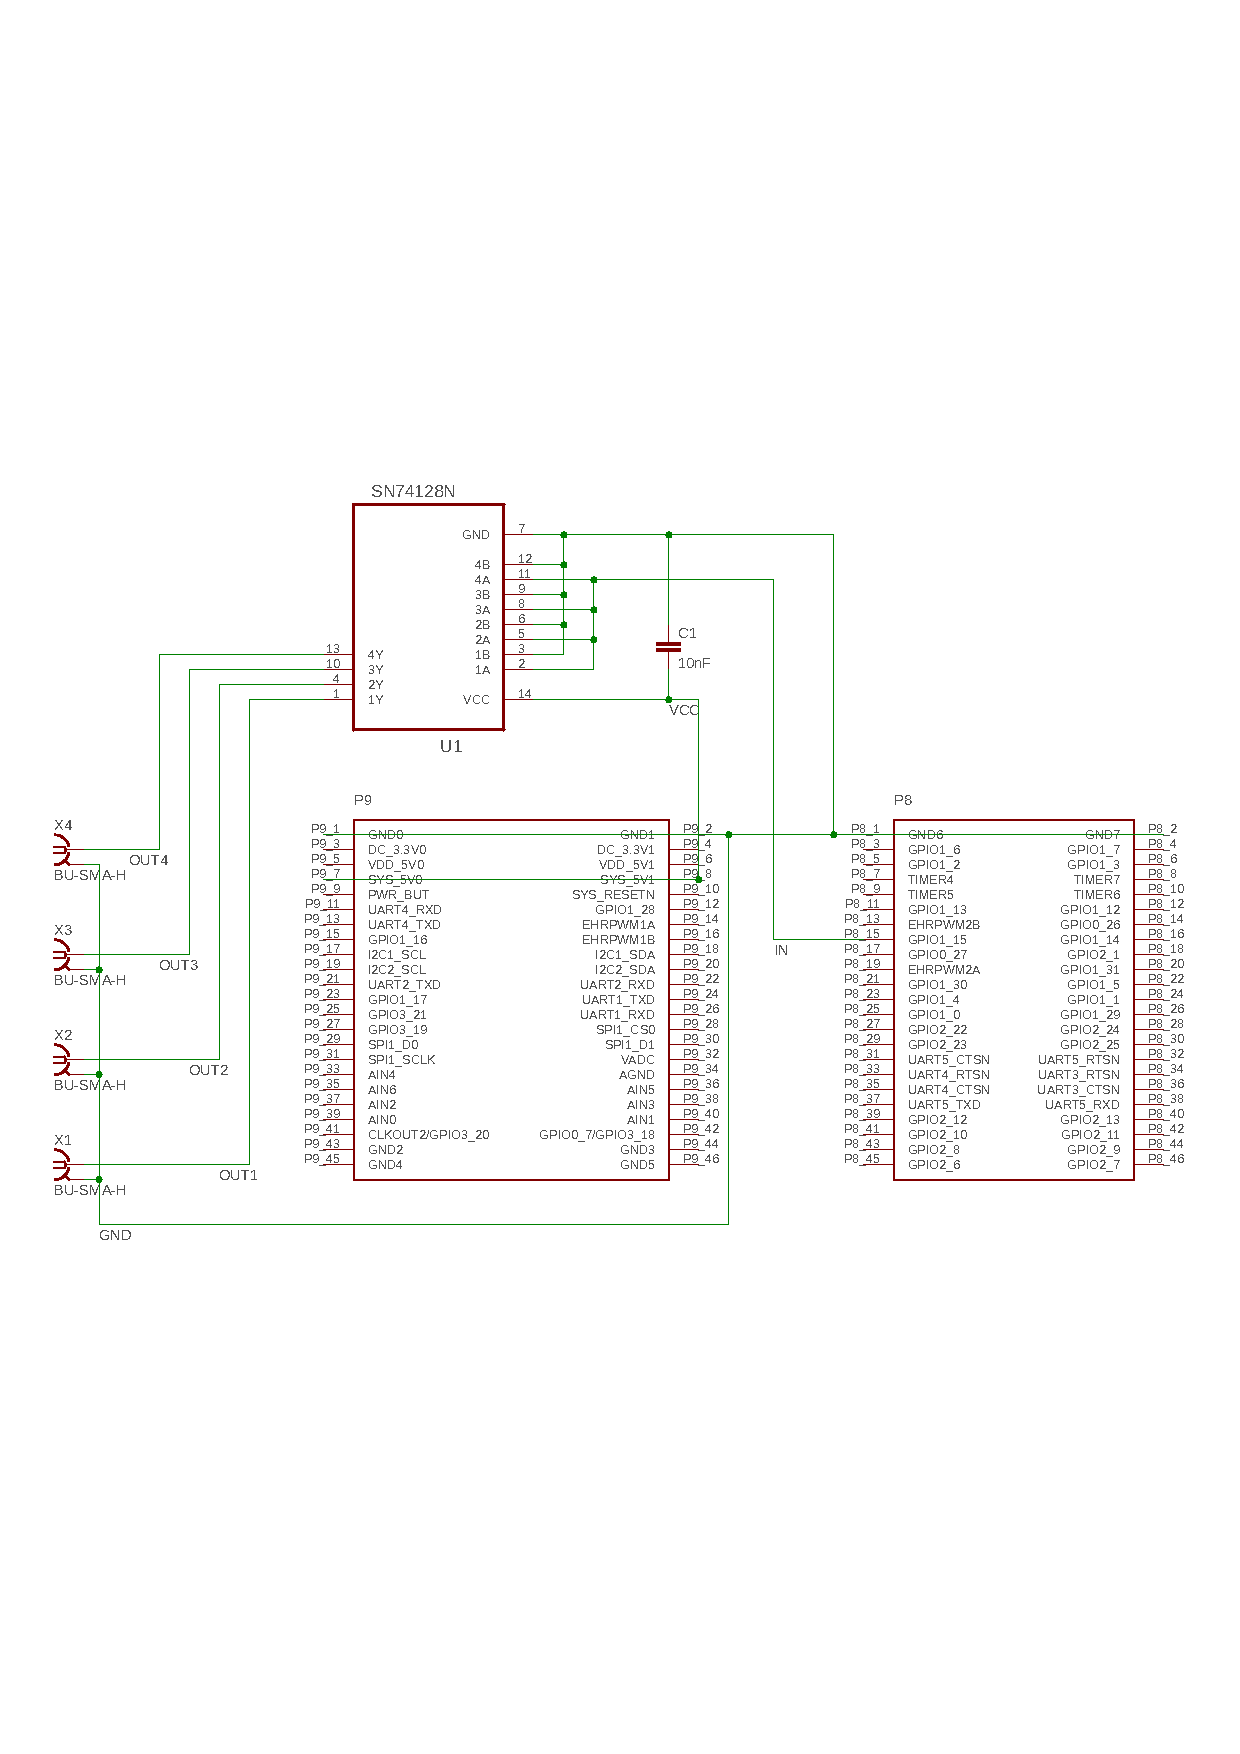
\includegraphics[width=\textwidth]{images/circuit/line-driver/scheme.pdf}
  \caption{Schematic of trigger source amplifier with digital input
  and four \gls{SMA} connectors.}
  \label{fig:elec:trig:scheme}
\end{figure}

\begin{figure}[h]
  \centering
  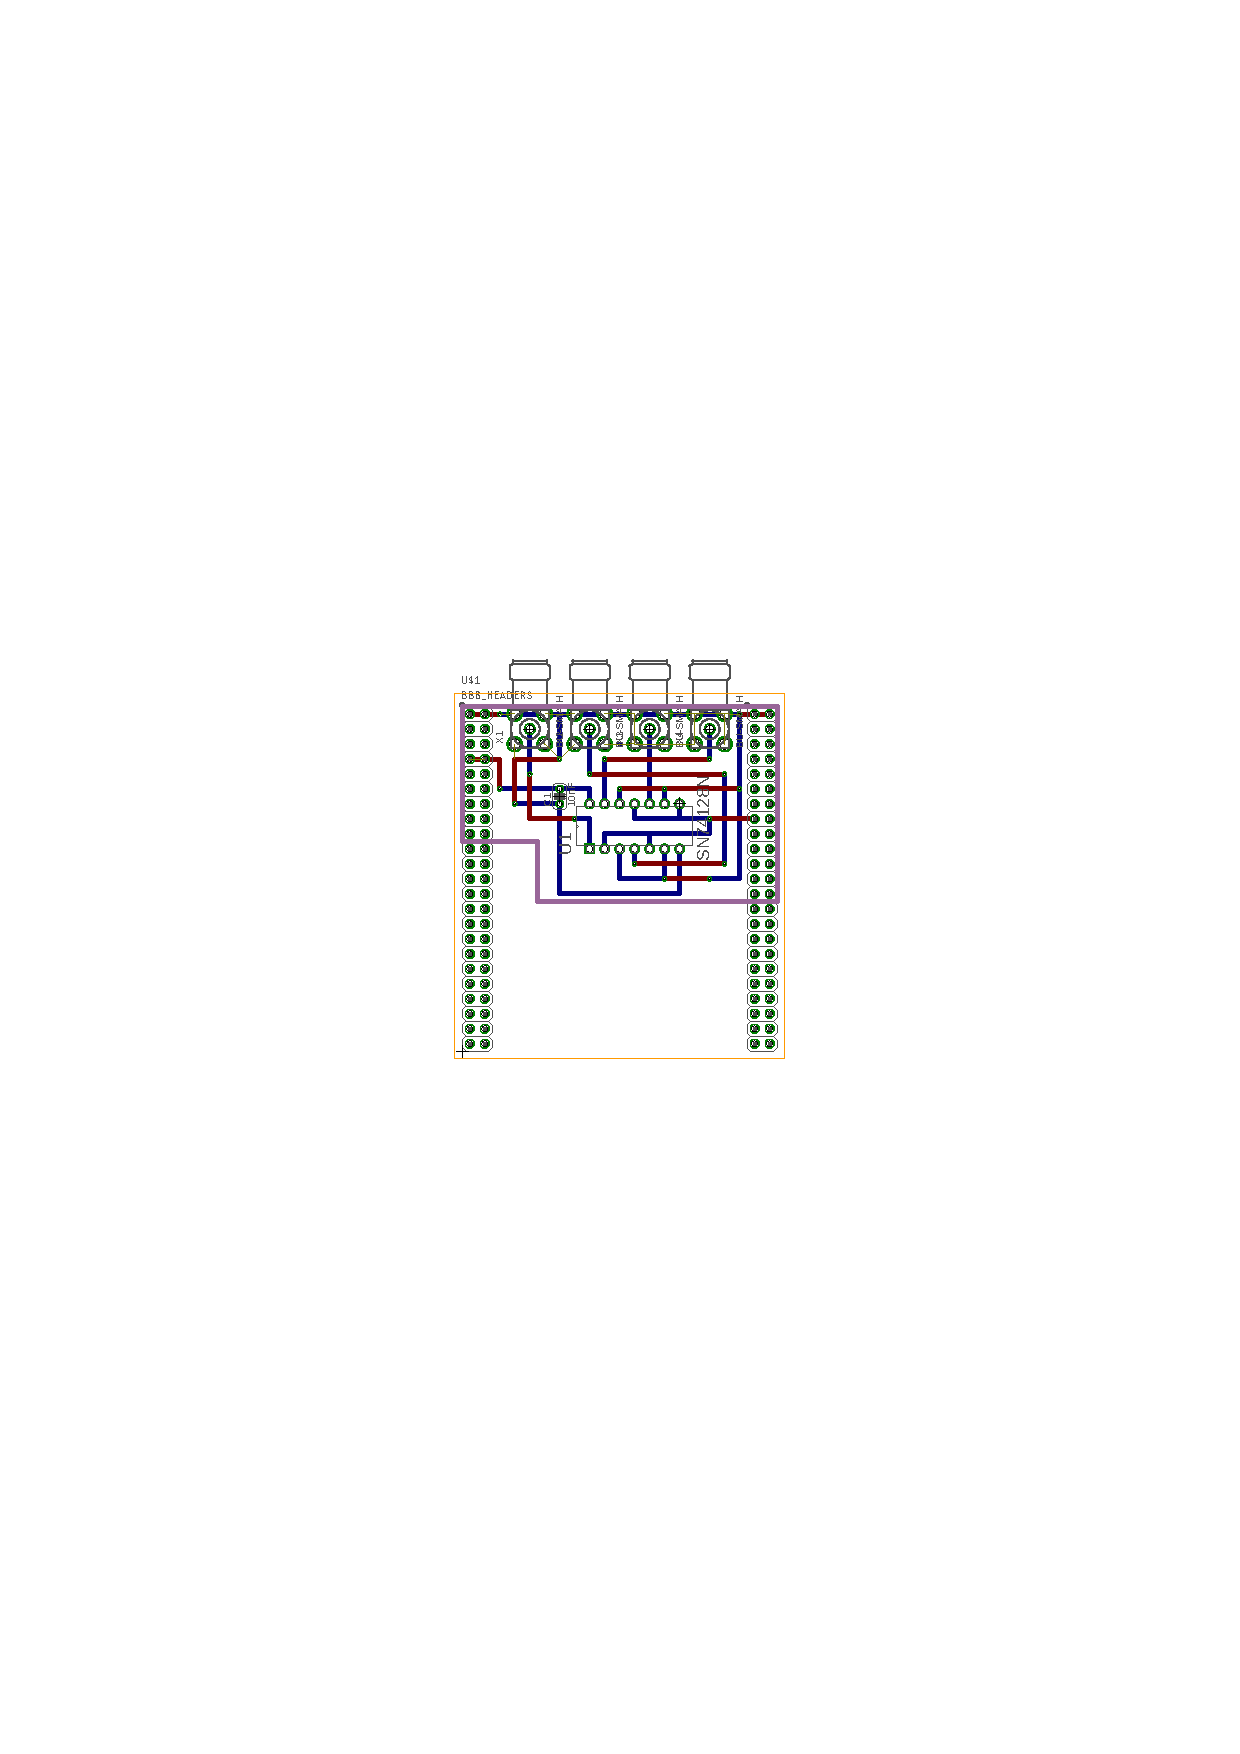
\includegraphics[width=.4\textwidth]{images/circuit/line-driver/board.pdf}
  \caption{Board layout of trigger source amplifier fitted to be mounted on
  top of the BeagleBone Black headers.}
  \label{fig:elec:trig:board}
\end{figure}
